\chapter{Mask R-CNN}
\noindent

\section{The problem with Faster R-CNN}
\noindent

	Until now, we know how Faster R-CNN extract feature maps by passing the image through lots of convolutional layer. However, while down sampling the image, we also scaled down the RoIs inside the image with a specific factor and round the offset of their bounding boxes. As a result, we create a new bounding box for the object inside which cause missing information and reduce performance of our system.
	
	An example below illustrates when we feed 512x512 image to VGG16 and cause quantization on bounding box offset. The blue part is the missing piece data and the one green is a new data created by quantization.
	
	\begin{figure}[H]
		\centering
		{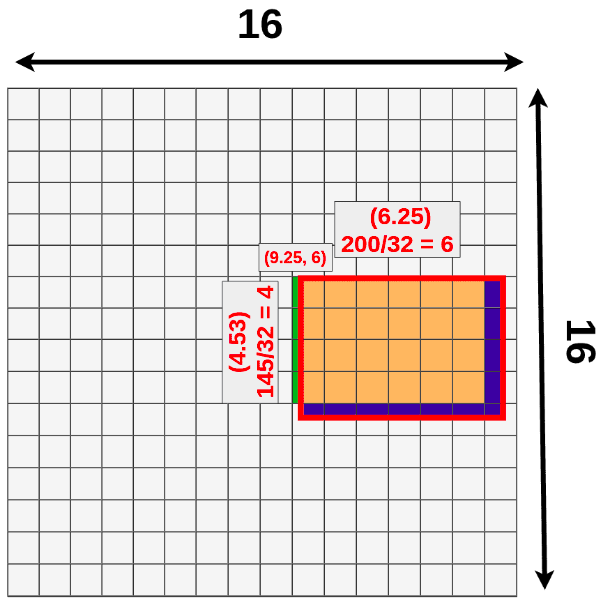
\includegraphics[width=0.4\textwidth]{./hinhanh/chap5/problem.png}}
		\caption{Example of quantization problem causing missing information.}
	\end{figure}
	
	As mention before in RoI pooling layer, RoI pooling operation will quantize floating number of RoI offset to a discrete offset. Then this quantized RoI is subdivided into spatial bins which are then aggregated (usually by max pooling) [5]. And once again, we lose vector information. We can look at Figure 7 for more details.

\section{An extended solving the problem - Mask R-CNN}
\noindent

	In 2017, a group of Facebook AI researchers - Kaiming He at el presented a new system which is influenced by Faster R-CNN called Mask R-CNN. This system, gennerally, is an extend of Faster R-CNN with a new branch for segmentation generating an object mask. Unlike others system which are complex multiple-stage cascade that predicts segment proposals from bounding-box proposals, followed by classification. Mask R-CNN allows three branches (including the existing branch for classification and bounding box regression, and a branch for predicting segmentation masks on RoI) to run in parallel which enhance the processing speed.	
	
	\begin{figure}[H]
		\centering
		{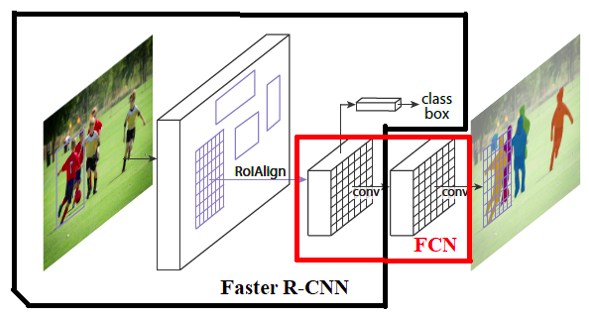
\includegraphics[width=0.6\textwidth]{./hinhanh/chap5/mask_rcnn.png}}
		\caption{Mask R-CNN architecture including Faster R-CNN and FCN}
	\end{figure}
	
	As Figure 8 shows that Mask R-CNN is constructed by Faster R-CNN and a small fully convolution neural network. Because it is a stack of convolutional layer, the mask branch only consumes a small computational resource enabling the system to run extremely fast in testing phrase just like Faster R-CNN speed (~0.2s/image). 
	
	It is noticeable that Mask R-CNN’s authors solved the problem of RoI Pooling quantization by proposing a brand-new alternative technique called RoI Align which completely secure spatial locations of bounding box and information inside it. According to the paper, this minor change can affect the result accuracy up to 50\%.
	
\subsection{Multi-task loss}
\noindent
	
	Inherit the spirit of Faster R-CNN, Mask R-CNN also has two stage procedure, with RPN is the first stage that generates proposals. In the next stage, in parallel with the original branch of Fast R-CNN, there is a mask generation branch that outputs a binary mask for each RoI. Therefore, a new loss function was proposed and defined as $ \L = L_{cls} + L_{box} + L_{mask}\ $. The classification and regression loss ($ \ L_{cls}, L_{box} \ $) are the same as those defined in \cite{fastrcnn}. 
	
	The mask loss, according to the authors, was defined as the average binary cross entropy loss (per-pixel sigmoid and binary loss) enabling the system to generate masks for each class without causing competition among them \cite{maskrcnn}. As a result, lots of masks will be generated but only the ground truth masks of class k in the corresponding RoIs are considered while calculating the mask loss (masks on another classes are not contribute to mask loss of class k). And by taking advantage of the classifier branch, the predicted class will be used to choose the output mask. This strategy decouples the mask and class prediction and outputs good instance segmentation results \cite{maskrcnn}. Therefore, Mask R-CNN’s strategy is different from most techniques at that time (in semantic segmentation problems) when adopting a per-pixel multinomial logistic loss and validate with the standard metric of mean pixel intersection over union (IoU), with the mean taken over all classes - softmax (competition between classes), including background \cite{maskrcnn}.






